\section{Object 2}
\markright{Object 2}

The construction of this object involved multiple features. The process began with a 2D sketch of the main body's profile, which was then extruded symmetrically using the "Mid Plane" end condition. Subsequently, a sketch for the top extension was created and extruded. The final step involved creating a sketch on the bottom face of the model and using the "Extruded Cut" feature to remove material and create the final shape.

\begin{figure}[H]
	\centering

	\begin{subfigure}[b]{0.49\textwidth}
		\centering
		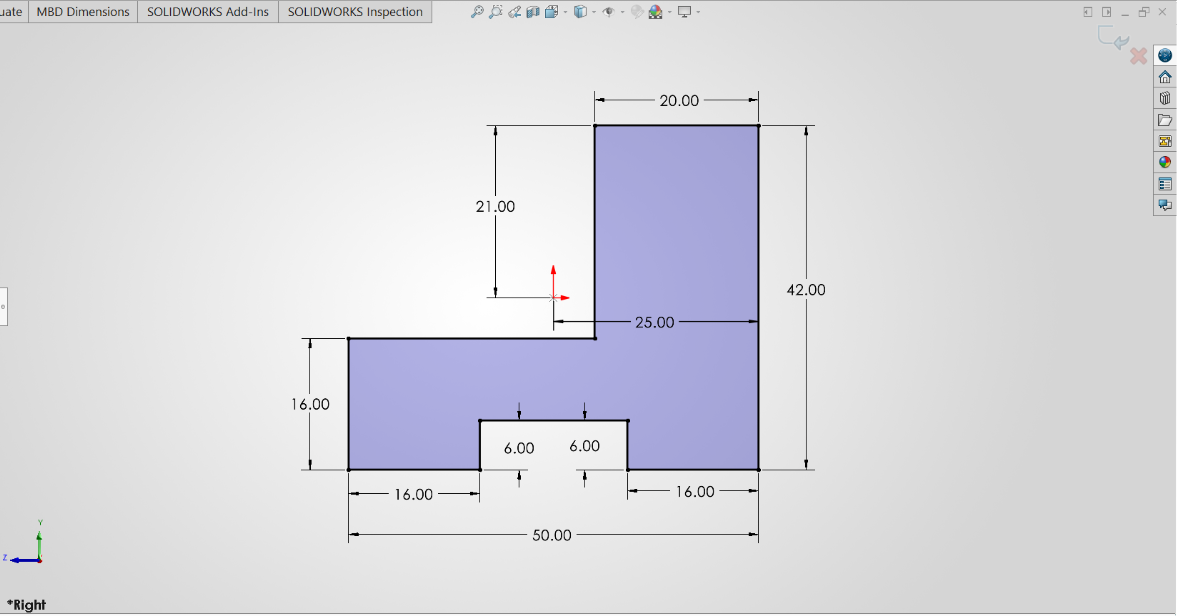
\includegraphics[width=\textwidth, keepaspectratio]{lab-01/assets/object-2/object-2-snap-1.png}
		\caption{2D drawing of the right view with dimentions}
	\end{subfigure}
	\hfill
	\begin{subfigure}[b]{0.49\textwidth}
		\centering
		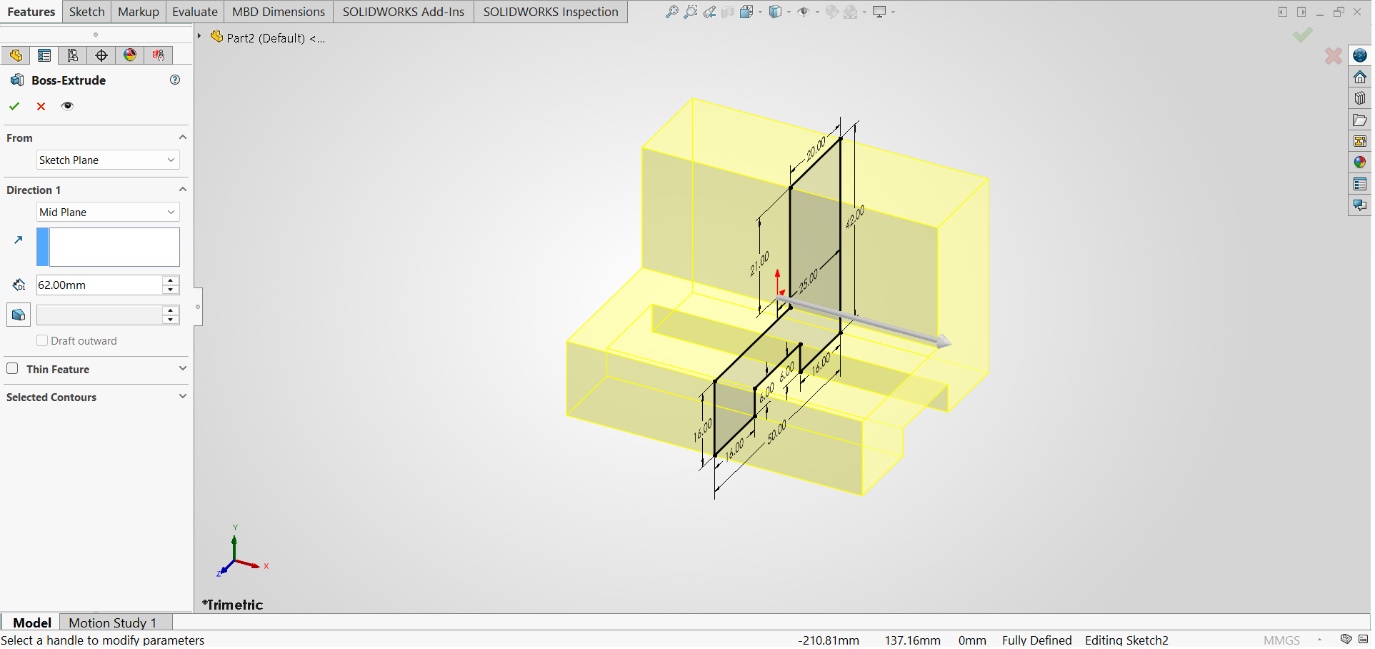
\includegraphics[width=\textwidth, keepaspectratio]{lab-01/assets/object-2/object-2-snap-2.png}
		\caption{Extruding from the midpoint}
	\end{subfigure}
	\begin{subfigure}[b]{0.49\textwidth}
		\centering
		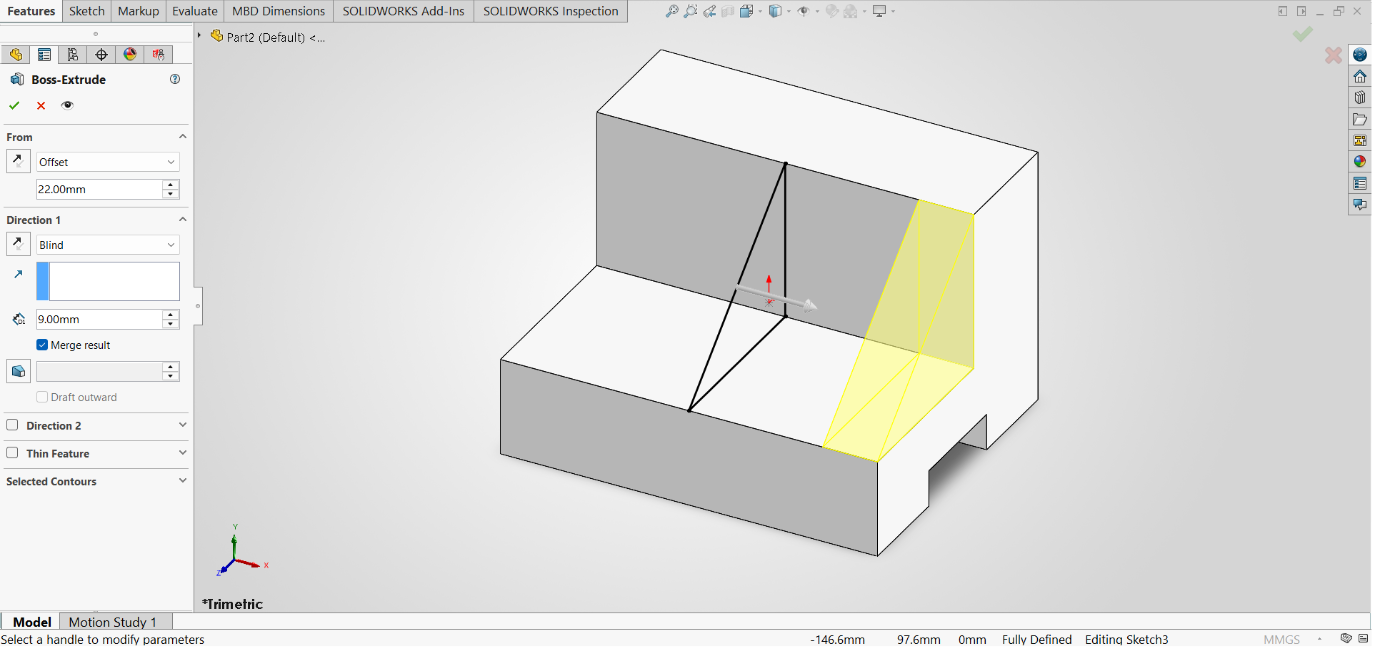
\includegraphics[width=\textwidth, keepaspectratio]{lab-01/assets/object-2/object-2-snap-5.png}
		\caption{Extruding the extension to the left}
	\end{subfigure}
	\hfill
	\begin{subfigure}[b]{0.49\textwidth}
		\centering
		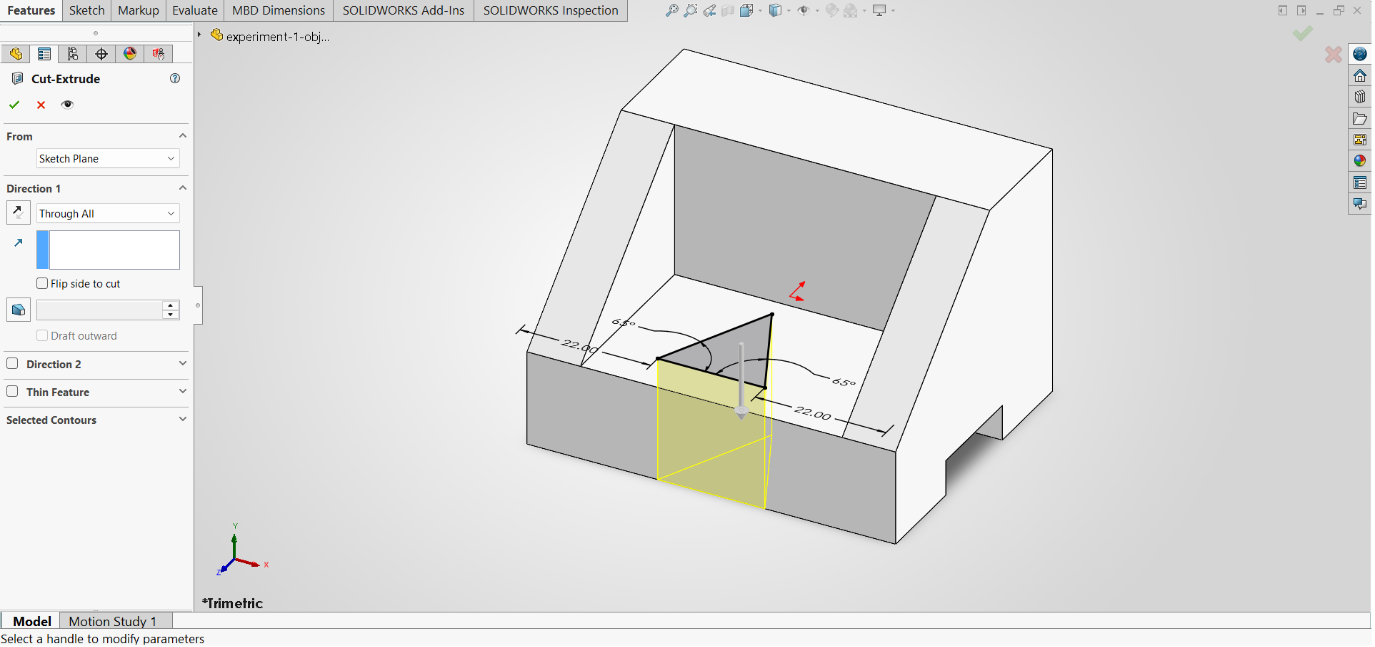
\includegraphics[width=\textwidth, keepaspectratio]{lab-01/assets/object-2/object-2-snap-10.png}
		\caption{Using extruded cut feature on the portion to be cut-off}
	\end{subfigure}
	\vspace{0.5em}
	\begin{subfigure}[b]{\textwidth}
		\centering
		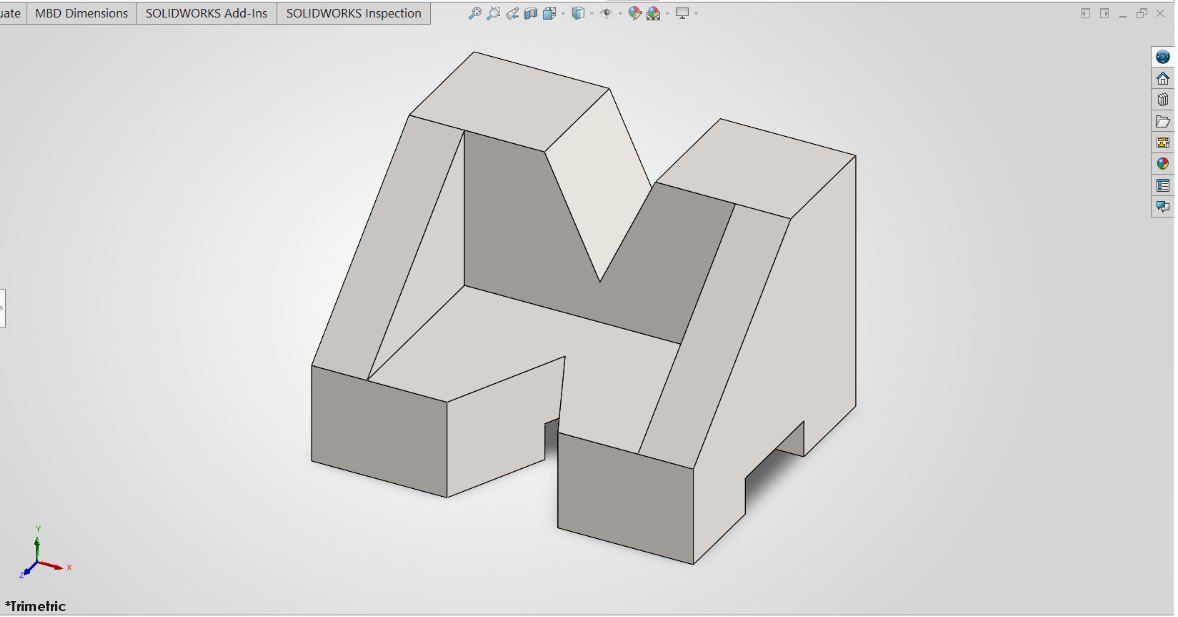
\includegraphics[width=\textwidth, keepaspectratio]{lab-01/assets/object-2/object-2-snap-14.png}
		\caption{Final result}
	\end{subfigure}

	\caption{Snapshots while Designing Object 2 in Solidworks}
	\label{lab01_object_2}
\end{figure}
